\documentclass{standalone}
\usepackage{tikz}
\usetikzlibrary{patterns, positioning}

\begin{document}
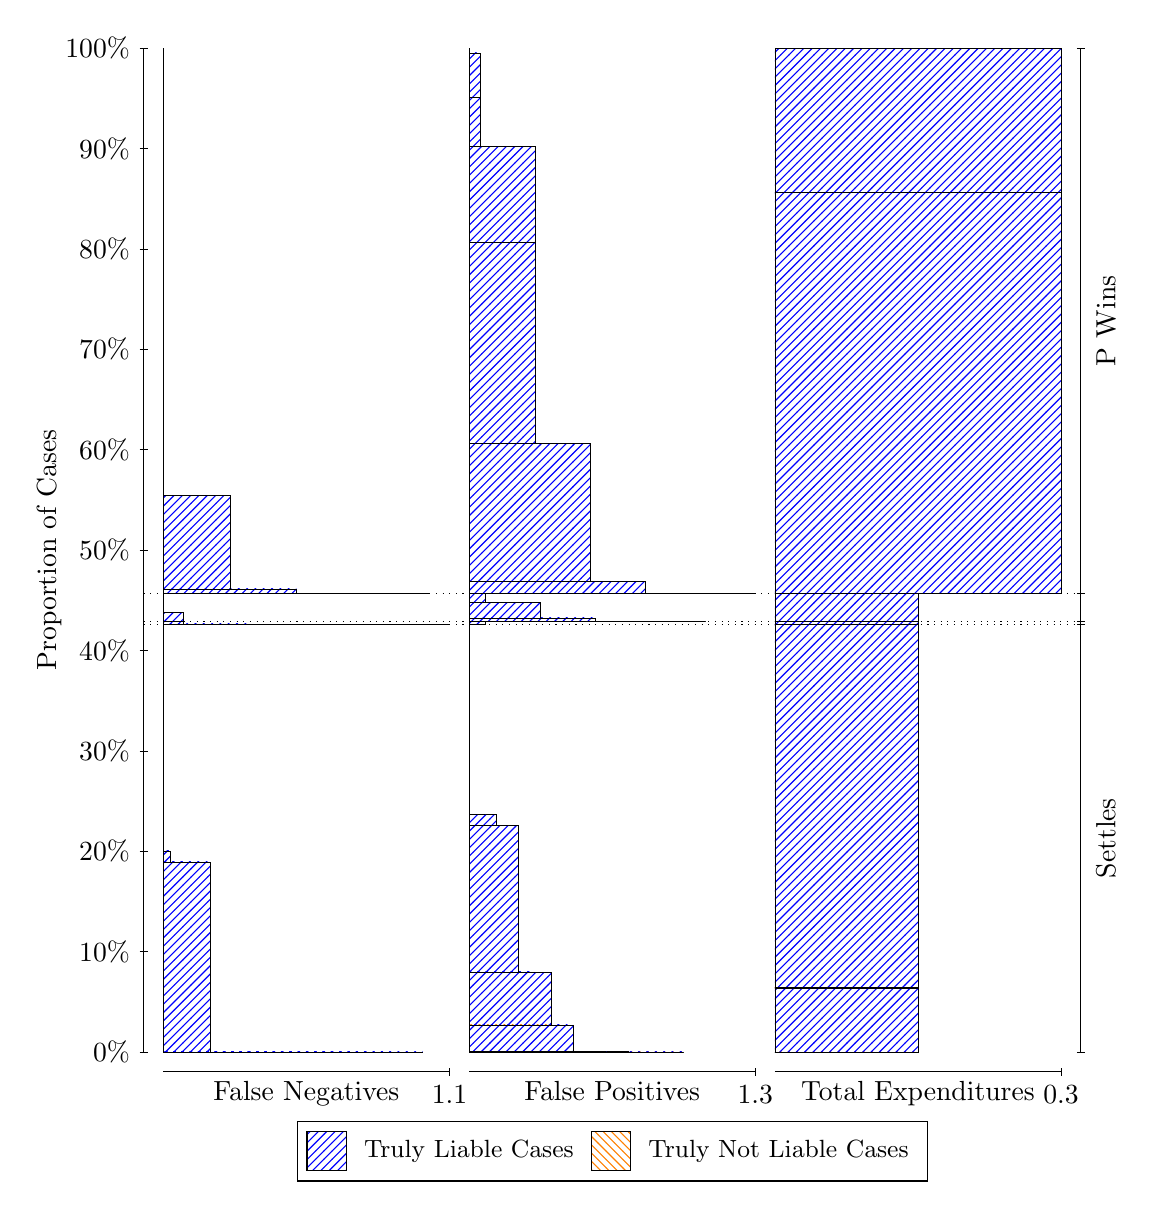
\begin{tikzpicture}
\draw[black, very thin] (1.5,1.75) -- (1.5,14.5);
\node[rotate=90, anchor=center] at (0.3, 8.125) {Proportion of Cases};
\draw[black, very thin] (1.45,1.75) -- (1.55,1.75);
\node[anchor=east] at (1.45, 1.75) {0\%};
\draw[black, very thin] (1.45,3.025) -- (1.55,3.025);
\node[anchor=east] at (1.45, 3.025) {10\%};
\draw[black, very thin] (1.45,4.3) -- (1.55,4.3);
\node[anchor=east] at (1.45, 4.3) {20\%};
\draw[black, very thin] (1.45,5.575) -- (1.55,5.575);
\node[anchor=east] at (1.45, 5.575) {30\%};
\draw[black, very thin] (1.45,6.85) -- (1.55,6.85);
\node[anchor=east] at (1.45, 6.85) {40\%};
\draw[black, very thin] (1.45,8.125) -- (1.55,8.125);
\node[anchor=east] at (1.45, 8.125) {50\%};
\draw[black, very thin] (1.45,9.4) -- (1.55,9.4);
\node[anchor=east] at (1.45, 9.4) {60\%};
\draw[black, very thin] (1.45,10.675) -- (1.55,10.675);
\node[anchor=east] at (1.45, 10.675) {70\%};
\draw[black, very thin] (1.45,11.95) -- (1.55,11.95);
\node[anchor=east] at (1.45, 11.95) {80\%};
\draw[black, very thin] (1.45,13.225) -- (1.55,13.225);
\node[anchor=east] at (1.45, 13.225) {90\%};
\draw[black, very thin] (1.45,14.5) -- (1.55,14.5);
\node[anchor=east] at (1.45, 14.5) {100\%};

\draw[black, very thin] (13.4,1.75) -- (13.4,14.5);
\draw[black, very thin] (13.35,1.75) -- (13.45,1.75);
\node[anchor=west] at (13.35, 1.75) {};
\draw[black, very thin] (13.35,7.1817) -- (13.45,7.1817);
\node[anchor=west] at (13.35, 7.1817) {};
\draw[black, very thin] (13.35,7.2203) -- (13.45,7.2203);
\node[anchor=west] at (13.35, 7.2203) {};
\draw[black, very thin] (13.35,7.5697) -- (13.45,7.5697);
\node[anchor=west] at (13.35, 7.5697) {};
\draw[black, very thin] (13.35,14.5) -- (13.45,14.5);
\node[anchor=west] at (13.35, 14.5) {};

\draw[black, very thin, pattern color=blue, pattern=north east lines] (1.75,1.75) rectangle (5.0453,1.75);
\draw[black, very thin, pattern color=blue, pattern=north east lines] (1.75,1.75) rectangle (4.7074,1.75);
\draw[black, very thin, pattern color=blue, pattern=north east lines] (1.75,1.75) rectangle (4.3694,1.75);
\draw[black, very thin, pattern color=blue, pattern=north east lines] (1.75,1.75) rectangle (4.2004,1.75);
\draw[black, very thin, pattern color=blue, pattern=north east lines] (1.75,1.75) rectangle (4.0314,1.75);
\draw[black, very thin, pattern color=blue, pattern=north east lines] (1.75,1.75) rectangle (3.8624,1.75);
\draw[black, very thin, pattern color=blue, pattern=north east lines] (1.75,1.75) rectangle (3.6934,1.75);
\draw[black, very thin, pattern color=blue, pattern=north east lines] (1.75,1.75) rectangle (3.5244,1.75);
\draw[black, very thin, pattern color=blue, pattern=north east lines] (1.75,1.75) rectangle (3.3554,1.75);
\draw[black, very thin, pattern color=blue, pattern=north east lines] (1.75,1.75) rectangle (3.1864,1.75);
\draw[black, very thin, pattern color=blue, pattern=north east lines] (1.75,1.75) rectangle (3.1864,1.75);
\draw[black, very thin, pattern color=blue, pattern=north east lines] (1.75,1.75) rectangle (3.0174,1.75);
\draw[black, very thin, pattern color=blue, pattern=north east lines] (1.75,1.75) rectangle (2.8484,1.75);
\draw[black, very thin, pattern color=blue, pattern=north east lines] (1.75,1.75) rectangle (2.6795,1.7513);
\draw[black, very thin, pattern color=blue, pattern=north east lines] (1.75,1.7513) rectangle (2.6795,1.7513);
\draw[black, very thin, pattern color=blue, pattern=north east lines] (1.75,1.7513) rectangle (2.5105,1.7519);
\draw[black, very thin, pattern color=blue, pattern=north east lines] (1.75,1.7519) rectangle (2.3415,1.7519);
\draw[black, very thin, pattern color=blue, pattern=north east lines] (1.75,1.7519) rectangle (2.3415,1.7519);
\draw[black, very thin, pattern color=blue, pattern=north east lines] (1.75,1.7519) rectangle (2.3415,4.1647);
\draw[black, very thin, pattern color=blue, pattern=north east lines] (1.75,4.1647) rectangle (2.1725,4.1655);
\draw[black, very thin, pattern color=blue, pattern=north east lines] (1.75,4.1655) rectangle (2.0035,4.1655);
\draw[black, very thin, pattern color=blue, pattern=north east lines] (1.75,4.1655) rectangle (1.8345,4.3045);
\draw[black, very thin, pattern color=blue, pattern=north east lines] (1.75,4.3045) rectangle (1.8345,4.3045);
\draw[black, very thin, pattern color=orange, pattern=north west lines] (1.75,4.3045) rectangle (1.75,4.3045);
\draw[black, very thin, pattern color=blue, pattern=north east lines] (1.75,4.3045) rectangle (1.75,7.1817);
\draw[black, very thin, pattern color=blue, pattern=north east lines] (1.75,7.1817) rectangle (5.3833,7.1817);
\draw[black, very thin, pattern color=blue, pattern=north east lines] (1.75,7.1817) rectangle (4.5384,7.1817);
\draw[black, very thin, pattern color=blue, pattern=north east lines] (1.75,7.1817) rectangle (3.6934,7.1817);
\draw[black, very thin, pattern color=blue, pattern=north east lines] (1.75,7.1817) rectangle (2.8484,7.1878);
\draw[black, very thin, pattern color=blue, pattern=north east lines] (1.75,7.1878) rectangle (2.0035,7.2203);
\draw[black, very thin, pattern color=orange, pattern=north west lines] (1.75,7.2203) rectangle (1.75,7.2203);
\draw[black, very thin, pattern color=blue, pattern=north east lines] (1.75,7.2203) rectangle (2.0035,7.3287);
\draw[black, very thin, pattern color=orange, pattern=north west lines] (1.75,7.3287) rectangle (1.75,7.3287);
\draw[black, very thin, pattern color=blue, pattern=north east lines] (1.75,7.3287) rectangle (1.75,7.5697);
\draw[black, very thin, pattern color=blue, pattern=north east lines] (1.75,7.5697) rectangle (5.1298,7.5697);
\draw[black, very thin, pattern color=blue, pattern=north east lines] (1.75,7.5697) rectangle (4.2849,7.5699);
\draw[black, very thin, pattern color=blue, pattern=north east lines] (1.75,7.5699) rectangle (3.4399,7.6304);
\draw[black, very thin, pattern color=blue, pattern=north east lines] (1.75,7.6304) rectangle (2.595,8.8178);
\draw[black, very thin, pattern color=orange, pattern=north west lines] (1.75,8.8178) rectangle (1.75,8.8178);
\draw[black, very thin, pattern color=blue, pattern=north east lines] (1.75,8.8178) rectangle (1.75,14.5);
\draw[black, very thin, pattern color=orange, pattern=north west lines] (5.6333,1.75) rectangle (8.3583,1.75);
\draw[black, very thin, pattern color=blue, pattern=north east lines] (5.6333,1.75) rectangle (8.3583,1.75);
\draw[black, very thin, pattern color=orange, pattern=north west lines] (5.6333,1.75) rectangle (8.0788,1.75);
\draw[black, very thin, pattern color=blue, pattern=north east lines] (5.6333,1.75) rectangle (8.0788,1.75);
\draw[black, very thin, pattern color=orange, pattern=north west lines] (5.6333,1.75) rectangle (7.7994,1.75);
\draw[black, very thin, pattern color=blue, pattern=north east lines] (5.6333,1.75) rectangle (7.7994,1.75);
\draw[black, very thin, pattern color=blue, pattern=north east lines] (5.6333,1.75) rectangle (7.6596,1.7526);
\draw[black, very thin, pattern color=orange, pattern=north west lines] (5.6333,1.7526) rectangle (7.5199,1.7526);
\draw[black, very thin, pattern color=blue, pattern=north east lines] (5.6333,1.7526) rectangle (7.5199,1.7526);
\draw[black, very thin, pattern color=blue, pattern=north east lines] (5.6333,1.7526) rectangle (7.3801,1.7526);
\draw[black, very thin, pattern color=orange, pattern=north west lines] (5.6333,1.7526) rectangle (7.2404,1.7526);
\draw[black, very thin, pattern color=blue, pattern=north east lines] (5.6333,1.7526) rectangle (7.2404,1.7526);
\draw[black, very thin, pattern color=blue, pattern=north east lines] (5.6333,1.7526) rectangle (7.1006,1.7526);
\draw[black, very thin, pattern color=orange, pattern=north west lines] (5.6333,1.7526) rectangle (6.9609,1.7526);
\draw[black, very thin, pattern color=blue, pattern=north east lines] (5.6333,1.7526) rectangle (6.9609,1.7527);
\draw[black, very thin, pattern color=orange, pattern=north west lines] (5.6333,1.7527) rectangle (6.9609,1.7527);
\draw[black, very thin, pattern color=blue, pattern=north east lines] (5.6333,1.7527) rectangle (6.9609,2.0932);
\draw[black, very thin, pattern color=blue, pattern=north east lines] (5.6333,2.0932) rectangle (6.8212,2.0935);
\draw[black, very thin, pattern color=orange, pattern=north west lines] (5.6333,2.0935) rectangle (6.6814,2.0935);
\draw[black, very thin, pattern color=blue, pattern=north east lines] (5.6333,2.0935) rectangle (6.6814,2.7626);
\draw[black, very thin, pattern color=blue, pattern=north east lines] (5.6333,2.7626) rectangle (6.5417,2.7626);
\draw[black, very thin, pattern color=orange, pattern=north west lines] (5.6333,2.7626) rectangle (6.4019,2.7626);
\draw[black, very thin, pattern color=blue, pattern=north east lines] (5.6333,2.7626) rectangle (6.4019,2.7666);
\draw[black, very thin, pattern color=blue, pattern=north east lines] (5.6333,2.7666) rectangle (6.4019,2.7666);
\draw[black, very thin, pattern color=blue, pattern=north east lines] (5.6333,2.7666) rectangle (6.2622,2.7667);
\draw[black, very thin, pattern color=blue, pattern=north east lines] (5.6333,2.7667) rectangle (6.2622,4.6237);
\draw[black, very thin, pattern color=orange, pattern=north west lines] (5.6333,4.6237) rectangle (6.1224,4.6237);
\draw[black, very thin, pattern color=blue, pattern=north east lines] (5.6333,4.6237) rectangle (6.1224,4.6269);
\draw[black, very thin, pattern color=blue, pattern=north east lines] (5.6333,4.6269) rectangle (6.1224,4.6272);
\draw[black, very thin, pattern color=blue, pattern=north east lines] (5.6333,4.6272) rectangle (5.9827,4.7662);
\draw[black, very thin, pattern color=blue, pattern=north east lines] (5.6333,4.7662) rectangle (5.8429,4.7662);
\draw[black, very thin, pattern color=blue, pattern=north east lines] (5.6333,4.7662) rectangle (5.7032,4.767);
\draw[black, very thin, pattern color=blue, pattern=north east lines] (5.6333,4.767) rectangle (5.7032,4.767);
\draw[black, very thin, pattern color=blue, pattern=north east lines] (5.6333,4.767) rectangle (5.6333,7.1817);
\draw[black, very thin, pattern color=orange, pattern=north west lines] (5.6333,7.1817) rectangle (5.8429,7.1817);
\draw[black, very thin, pattern color=blue, pattern=north east lines] (5.6333,7.1817) rectangle (5.8429,7.2142);
\draw[black, very thin, pattern color=blue, pattern=north east lines] (5.6333,7.2142) rectangle (5.6333,7.2203);
\draw[black, very thin, pattern color=orange, pattern=north west lines] (5.6333,7.2203) rectangle (8.6378,7.2203);
\draw[black, very thin, pattern color=blue, pattern=north east lines] (5.6333,7.2203) rectangle (8.6378,7.2203);
\draw[black, very thin, pattern color=blue, pattern=north east lines] (5.6333,7.2203) rectangle (7.9391,7.2206);
\draw[black, very thin, pattern color=blue, pattern=north east lines] (5.6333,7.2206) rectangle (7.2404,7.2636);
\draw[black, very thin, pattern color=blue, pattern=north east lines] (5.6333,7.2636) rectangle (6.5417,7.4613);
\draw[black, very thin, pattern color=blue, pattern=north east lines] (5.6333,7.4613) rectangle (5.8429,7.5697);
\draw[black, very thin, pattern color=orange, pattern=north west lines] (5.6333,7.5697) rectangle (9.2667,7.5697);
\draw[black, very thin, pattern color=blue, pattern=north east lines] (5.6333,7.5697) rectangle (9.2667,7.5697);
\draw[black, very thin, pattern color=orange, pattern=north west lines] (5.6333,7.5697) rectangle (8.5679,7.5697);
\draw[black, very thin, pattern color=blue, pattern=north east lines] (5.6333,7.5697) rectangle (8.5679,7.5718);
\draw[black, very thin, pattern color=orange, pattern=north west lines] (5.6333,7.5718) rectangle (7.8692,7.5718);
\draw[black, very thin, pattern color=blue, pattern=north east lines] (5.6333,7.5718) rectangle (7.8692,7.7299);
\draw[black, very thin, pattern color=orange, pattern=north west lines] (5.6333,7.7299) rectangle (7.1705,7.7299);
\draw[black, very thin, pattern color=blue, pattern=north east lines] (5.6333,7.7299) rectangle (7.1705,9.4743);
\draw[black, very thin, pattern color=blue, pattern=north east lines] (5.6333,9.4743) rectangle (6.4718,12.033);
\draw[black, very thin, pattern color=orange, pattern=north west lines] (5.6333,12.033) rectangle (6.4718,12.033);
\draw[black, very thin, pattern color=blue, pattern=north east lines] (5.6333,12.033) rectangle (6.4718,13.252);
\draw[black, very thin, pattern color=blue, pattern=north east lines] (5.6333,13.252) rectangle (5.7731,13.875);
\draw[black, very thin, pattern color=blue, pattern=north east lines] (5.6333,13.875) rectangle (5.7731,14.439);
\draw[black, very thin, pattern color=blue, pattern=north east lines] (5.6333,14.439) rectangle (5.6333,14.5);
\draw[black, very thin, pattern color=orange, pattern=north west lines] (9.5167,1.75) rectangle (11.333,1.75);
\draw[black, very thin, pattern color=blue, pattern=north east lines] (9.5167,1.75) rectangle (11.333,2.5644);
\draw[black, very thin, pattern color=orange, pattern=north west lines] (9.5167,2.5644) rectangle (11.333,2.5644);
\draw[black, very thin, pattern color=blue, pattern=north east lines] (9.5167,2.5644) rectangle (11.333,2.5682);
\draw[black, very thin, pattern color=orange, pattern=north west lines] (9.5167,2.5682) rectangle (11.333,2.5682);
\draw[black, very thin, pattern color=blue, pattern=north east lines] (9.5167,2.5682) rectangle (11.333,7.1817);
\draw[black, very thin, pattern color=orange, pattern=north west lines] (9.5167,7.1817) rectangle (11.333,7.1817);
\draw[black, very thin, pattern color=blue, pattern=north east lines] (9.5167,7.1817) rectangle (11.333,7.2203);
\draw[black, very thin, pattern color=orange, pattern=north west lines] (9.5167,7.2203) rectangle (11.333,7.2203);
\draw[black, very thin, pattern color=blue, pattern=north east lines] (9.5167,7.2203) rectangle (11.333,7.5697);
\draw[black, very thin, pattern color=orange, pattern=north west lines] (9.5167,7.5697) rectangle (13.15,7.5697);
\draw[black, very thin, pattern color=blue, pattern=north east lines] (9.5167,7.5697) rectangle (13.15,12.668);
\draw[black, very thin, pattern color=orange, pattern=north west lines] (9.5167,12.668) rectangle (13.15,12.668);
\draw[black, very thin, pattern color=blue, pattern=north east lines] (9.5167,12.668) rectangle (13.15,14.5);
\draw[black, dotted] (1.5,7.1817) -- (13.4,7.1817);
\draw[black, dotted] (1.5,7.2203) -- (13.4,7.2203);
\draw[black, dotted] (1.5,7.5697) -- (13.4,7.5697);
\draw[black, very thin] (1.75,1.5) -- (5.3833,1.5);
\node[anchor=north] at (3.5667, 1.5) {False Negatives};
\draw[black, very thin] (5.3833,1.45) -- (5.3833,1.55);
\node[anchor=north] at (5.3833, 1.45) {1.1};

\draw[black, very thin] (5.6333,1.5) -- (9.2667,1.5);
\node[anchor=north] at (7.45, 1.5) {False Positives};
\draw[black, very thin] (9.2667,1.45) -- (9.2667,1.55);
\node[anchor=north] at (9.2667, 1.45) {1.3};

\draw[black, very thin] (9.5167,1.5) -- (13.15,1.5);
\node[anchor=north] at (11.333, 1.5) {Total Expenditures};
\draw[black, very thin] (13.15,1.45) -- (13.15,1.55);
\node[anchor=north] at (13.15, 1.45) {0.3};

\node[black, centered, rotate=90] at (13.72, 4.4658) {Settles};


\node[black, centered, rotate=90] at (13.72, 11.035) {P Wins};

\draw (7.449999999999999,1.5) node[draw=none] (baseCoordinate) {};
\begin{scope}[align=center]
        \matrix[scale=0.5, draw=black, below=0.5cm of baseCoordinate, nodes={draw}, column sep=0.1cm]{
            \node[rectangle, draw, minimum width=0.5cm, minimum height=0.5cm, pattern=north east lines, pattern color=blue] {}; &
            \node[draw=none, font=\small] (B) {Truly Liable Cases}; &
            \node[rectangle, draw, minimum width=0.5cm, minimum height=0.5cm, pattern=north west lines, pattern color=orange] {}; &
            \node[draw=none, font=\small] (B) {Truly Not Liable Cases}; \\
            };
\end{scope}

\end{tikzpicture}
\end{document}